% TASK bpsi->kyoshimi merge & TRX->tr consolidation -- academic Beamer deck.
% Build:  pdflatex 2026-06-30-merge-trx-beamer.tex   (run twice for the outline/refs)
% Standard packages only (beamer, booktabs, amsmath, tikz) -- no external theme needed.
\documentclass[10pt,aspectratio=169]{beamer}
\usetheme{Madrid}
\usecolortheme{seahorse}
\usepackage[T1]{fontenc}
\usepackage[utf8]{inputenc}
\usepackage{booktabs}
\usepackage{amsmath,amssymb}
\usepackage{xcolor}
\usepackage{tikz}
\usetikzlibrary{arrows.meta,positioning}

\definecolor{ok}{RGB}{15,110,86}
\definecolor{warn}{RGB}{186,117,23}
\newcommand{\C}[1]{\texttt{\small #1}}          % inline code (escape _ inside!)
\newcommand{\good}{\textcolor{ok}{\textbf{green}}}
\hypersetup{colorlinks=true, urlcolor=blue!60!black, linkcolor=black}   % beamer loads hyperref

\title[TASK merge \& TRX port]{Merging upstream \texttt{bpsi} into a modernized TASK fork\\
and consolidating \textsc{trx} $\to$ \texttt{tr}}
\subtitle{Engineering report and lessons learned}
\author{TASK modernization effort}
\institute[]{Plasma simulation stack --- P0 merge (delivered) + P1 fusion port (in progress)}
\date{2026-06-30}

\begin{document}

\begin{frame}[plain]\titlepage\end{frame}

\begin{frame}{Outline}\tableofcontents\end{frame}

% ---------------------------------------------------------------
\section{Background}
\begin{frame}{Background: three git lines that had drifted apart}
\textbf{TASK} --- a Fortran tokamak transport stack (\C{eq}, \C{tr}/\C{trx},
\C{fp}, \C{wr}/\C{wrx}, \C{wm}, \C{tot} orchestrator, \dots).
\vspace{0.6em}
\begin{table}\footnotesize
\begin{tabular}{@{}lll@{}}
\toprule
Line & Origin & Role \\
\midrule
\textbf{bpsi} & Kyoto main dev & latest physics + bug-fixes (the base) \\
\textbf{kyoshimi-develop} & fork of bpsi @ \C{8eed6fc2} & \textbf{Phase-L modernization} \\
\textbf{ats-fukuyama} & GitHub & stale 2023 backup (read-only) \\
\bottomrule
\end{tabular}
\end{table}
\vspace{0.4em}
\textbf{Phase-L} = F90-ification, per-module C-ABI + \C{libXapi.so} + Python wrappers + MCP
servers, and \C{trcomm} split into 6 sub-modules.
\vspace{0.6em}

\begin{block}{Goal --- one reliable baseline for many developers}
\textbf{Unify} the GitHub-hosted fork line (\C{kyoshimi-develop}) and the Kyoto main-dev line (\C{bpsi}) into a
\emph{single, CI-validated, reliable baseline} that different developers can branch from for
\emph{subsequent merges and new features} --- without regression. Then make \C{tr} the single
canonical transport module by porting \textsc{trx}'s newer fusion physics.
\end{block}
\end{frame}

% ---------------------------------------------------------------
\section{Motivation}
\begin{frame}{Why: converge two diverged lines into one reliable baseline}
\begin{center}
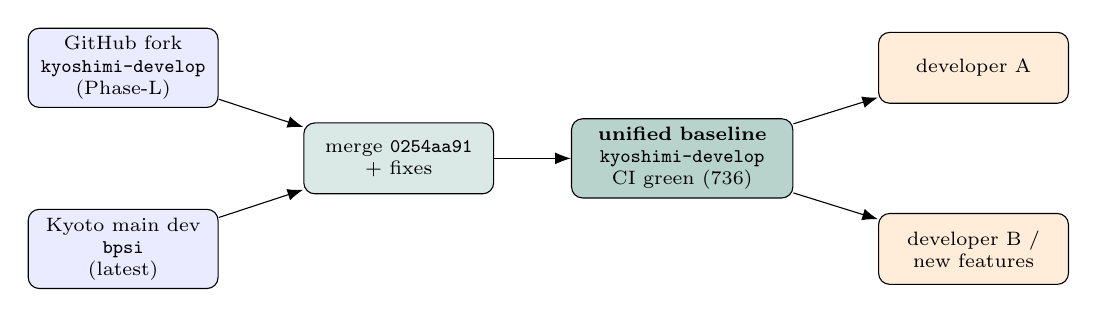
\begin{tikzpicture}[>={Latex[length=2mm]},
  box/.style={draw, rounded corners, align=center, inner sep=3pt, font=\scriptsize,
              minimum height=9mm, text width=22mm}]
  \node[box, fill=blue!8]                  (gh) at (0, 1.15) {GitHub fork\\ \texttt{kyoshimi-develop}\\ (Phase-L)};
  \node[box, fill=blue!8]                  (ky) at (0,-1.15) {Kyoto main dev\\ \texttt{bpsi}\\ (latest)};
  \node[box, fill=ok!15]                   (mg) at (3.5, 0)  {merge \texttt{0254aa91}\\ + fixes};
  \node[box, fill=ok!30, text width=26mm]  (bs) at (7.1, 0)  {\textbf{unified baseline}\\ \texttt{kyoshimi-develop}\\ CI green (736)};
  \node[box, fill=orange!15]               (dA) at (10.8, 1.15) {developer A};
  \node[box, fill=orange!15]               (dB) at (10.8,-1.15) {developer B /\\ new features};
  \draw[->] (gh) -- (mg);  \draw[->] (ky) -- (mg);
  \draw[->] (mg) -- (bs);
  \draw[->] (bs) -- (dA);  \draw[->] (bs) -- (dB);
\end{tikzpicture}
\end{center}
\textbf{Purpose:} unify the GitHub-hosted modernization (the Phase-L fork \texttt{kyoshimi-develop},
forked from \texttt{ats-fukuyama}) and the Kyoto \texttt{bpsi} line into \emph{one CI-validated, reliable
baseline} that developers branch from for subsequent merges and new features --- instead of
re-reconciling divergent trees each time. (The stale \texttt{ats-fukuyama} backup itself is superseded,
not a merge input.)
\end{frame}

% ---------------------------------------------------------------
\section{P0 --- the merge}
\begin{frame}[fragile]{P0: base selection and topology}
An audit found \C{bpsi/develop} is the latest base --- \emph{not} a 3-way upstream merge
(\C{ats-fukuyama} is 119 commits behind; its "unique" commits are superseded backups).

\begin{block}{Merge = bpsi base $\rightarrow$ the Phase-L fork}
\footnotesize
\begin{verbatim}
8eed6fc2  fork point (2025-12-16)
   |- bpsi/develop      +23 commits -> fa9dd493   (latest base)
   |- kyoshimi-develop  +Phase-L    -> 58f1fe2e   (C-ABI/.so/MCP/split)
        0254aa91 = merge(1st parent = fork, 2nd = bpsi base)
        + integration & baseline fixes -> d1f7f9e7  (CI green, delivered)
\end{verbatim}
\end{block}
Principle for every conflict: \textbf{keep the kyoshimi modernization, graft the bpsi intent}
(bug-fixes + the \C{eq}/\C{tr} q-solver refinement).
\end{frame}

\begin{frame}{P0: the 10 conflict resolutions}
\begin{table}\scriptsize
\begin{tabular}{@{}ll@{}}
\toprule
File & Resolution \\
\midrule
\C{eq/eqinit.f90} & graft into free-form: \C{NTVMAX} 200$\to$400, \C{NLPMAX} 20$\to$100 \\
\C{eq/eqcalc.f90} & graft bpsi \C{EQLOOP} adaptive under-relaxation \\
\C{eq/eqcalq.f90} & graft \C{NPRINT} print + \C{NMAX} 200$\to$400 \\
\C{eq/eqsub.f90}  & fixed-form $\to$ free-form; richer diagnostic \\
\C{pl/Makefile}   & keep \C{noeqlib} + take bpsi \C{SRCS\_NOEQ} + \C{plview.f90} \\
\C{tr/trcomm.f90} & take-ours (6-module split) + idempotent \C{DEALLOCATE\_TRCOMM} \\
\C{tr/trcomm\_param.f90} & species param list 8 $\to$ 15 \\
\C{tr/trmain.f90} & take-theirs (drop double-free) \\
\C{txnew/txcalv.f90} & take-theirs (SAVE-workspace) \\
\C{wrx/wrcalpwr.f90} & 3-way blend: keep headless/OOB clamp + graft \C{dx} \\
\bottomrule
\end{tabular}
\end{table}
\end{frame}

% ---------------------------------------------------------------
\section{Validation}
\begin{frame}{Getting CI to \good: issues surfaced class by class}
CI had \textbf{never} been green (even the pure base --- the build never reached pytest).
\begin{table}\scriptsize
\begin{tabular}{@{}ll@{}}
\toprule
Fix & Problem exposed \\
\midrule
\C{35c4bb5f}/\C{4bceac38} & eq fixed-form leak; lost wrx OOB clamp (auto-merge artifacts) \\
\C{4df6e541} & wrx \C{dx} $\div 0$; \C{trmain} dropped \C{USE}; non-idempotent dealloc \\
\C{d4afbaca} & \C{../task/make.header} not found (repo not named \C{task}) \\
\C{17f21f2c}/\C{9242c127} & bpsi added a bare \C{PT} to \C{plcomm\_parm} (ti/wm clash); \\
                          & \C{pl\_view} moved plparm$\to$plview (fp broke at \emph{link} time) \\
\C{bacf3f19} & numpy missing; mcp-servers not on \C{PYTHONPATH} (latent env gaps) \\
capture + \C{d1f7f9e7} & 3 equivalence baselines drift on gf13.2 (see next) \\
\bottomrule
\end{tabular}
\end{table}
\begin{center}\textbf{Result: 736 passed, 1 pre-existing xfail --- CI \good{} (py3.11 + 3.13).}\end{center}
Delivered by fast-forwarding \C{myfork/kyoshimi-develop} to \C{d1f7f9e7}.
\end{frame}

\begin{frame}{The 1e-10 equivalence baselines}
Three baselines drifted on the CI compiler (gfortran-13.2); \textbf{two distinct causes}:
\begin{itemize}
\item \C{wrx\_demo} / \C{wrx\_iter01} --- \textbf{compiler-version} FP reordering
      (gf8.5 $\ne$ gf13.2 $\ne$ gf15, all within $\sim$1e-9).
\item \C{tot\_ht6m\_short} --- a real $\sim$1e-4 \textbf{physics} shift (next slide).
\end{itemize}
\begin{alertblock}{Lesson}
1e-10 binary equivalence is too tight for FP-heavy modules (ray tracing, Fokker--Planck)
\emph{across compiler versions}, not just architectures --- capture baselines on the exact CI
compiler, or use a per-platform tolerance.
\end{alertblock}
Mechanism: an \emph{env-gated capture} dumps each case's gf13.2 \C{actual} metrics as a CI artifact;
those values are committed as the new baselines.
\end{frame}

% ---------------------------------------------------------------
\section{Case study: \texttt{tot\_ht6m}}
\begin{frame}{Case study: the \texttt{tot\_ht6m} q-solver refinement}
Root cause: bpsi's EQ-solver refinements --- finer flux-surface grid (\C{NMAX} 200$\to$400)
+ \C{EQLOOP} under-relaxation --- on the \C{modelg=3} \C{eq\_load} path.
\medskip

Signature (all 50 radial rows):
\begin{itemize}
\item current profile \textbf{redistributes} ($j$: $+$core, $-$mid to $-7.9$e-4 @ $\rho{=}0.74$,
      $+$edge; $q$ is its integral: $-$core, $+$outer);
\item \textbf{total current conserved} ($\Delta$\C{AJT} $=3.9$e-5 $\ll$ local $\Delta\,7.9$e-4);
\item \textbf{density frozen} (0/50 rows); smooth, no NaN.
\end{itemize}
\medskip
$\Rightarrow$ owner-approved as an intended higher-accuracy solve; baseline regenerated on gf13.2.
\end{frame}

\begin{frame}{Case study: a genuine review save}
\begin{alertblock}{Truncated tool output misleads}
An early analysis called the shift \emph{core-localized} ($\rho\le0.20$, zero beyond) --- an artifact
of a \textbf{truncated CI log} (the comparator prints only $\sim$52 of 210 mismatches, which happen to
be the core rows). Two independent pre-push reviewers caught the contradiction against the full
committed baseline; it was corrected to a \emph{global} redistribution and re-approved.
\end{alertblock}
\begin{block}{Takeaway}
Verify conclusions against the \emph{complete} data, and keep an independent-reviewer gate ---
it caught three real issues the author missed (the link-time \C{\_pl\_view\_}, a wrong root-cause
attribution, and this localization error).
\end{block}
\end{frame}

% ---------------------------------------------------------------
\section{P1 --- TRX $\to$ tr}
\begin{frame}{P1: old vs new fusion physics}
\begin{table}\footnotesize
\begin{tabular}{@{}lll@{}}
\toprule
 & kyoshimi \C{tr} (old) & bpsi \C{trx} (new) \\
\midrule
Selector    & scalar \C{MDLNF} & \C{model\_pnf} \\
Reactions   & hardcoded D+T (\C{TRNFDT}) & DT/DD/DHe3/TT/THe3 (\C{libnf}) \\
Source array& 1-D \C{SNF(NR)} & \C{SNF\_NSNNFNR(NS,NNF,NR)} \\
Reactivity  & analytic \C{SIGMAM(T)} & spline over tabulated \C{svnf\_*} \\
\bottomrule
\end{tabular}
\end{table}
\medskip
Recon corrected a plan premise: \C{tr\_m0904} / \C{tr\_iter01} \textbf{run \C{MDLNF=1}} (fusion ON),
so naively retiring \C{MDLNF} would change two core baselines. A direct physics comparison settled
the strategy.
\end{frame}

\begin{frame}{P1: the reactivity comparison drives the decision}
The old analytic DT reactivity:
\[
\langle\sigma v\rangle_{DT}=3.7\times10^{-18}\;T_I^{-2/3}\,
\frac{\exp\!\left(-20/T_I^{1/3}\right)}{H(T_I)},\qquad
T_I=\tfrac{3T_D+2T_T}{5}.
\]
\begin{block}{Finding}
The new \C{libnf} table \C{svnf\_dt} tabulates this same \C{SIGMAM} fit to 2 significant figures
(units: cm$^3$/s vs m$^3$/s). At the table points they agree to $0.03$--$1.2\%$. \C{libnf} splines the
\emph{raw} $\langle\sigma v\rangle$ vs $\log_{10}T$, so at core/fusion temperatures $T\gtrsim5$\,keV it
stays within $\sim$1--2\% of \C{SIGMAM}; between the low-$T$ edge points ($T\lesssim3$\,keV, where $\langle\sigma v\rangle$
is negligible) the raw-value spline deviates strongly --- immaterial to the fusion power.
\end{block}
$\Rightarrow$ migrating DT to \C{model\_pnf} gains \textbf{zero physics} at the core (the analytic
\C{MDLNF} is actually smoother); \C{model\_pnf}'s value is the \textbf{multi-reaction} capability
(DD/DHe3/TT/THe3), which is additive.
\end{frame}

\begin{frame}{P1: decision (Option A) and remaining plan}
\begin{block}{Decision --- Option A}
Keep the exact old \C{MDLNF}/\C{SIGMAM} DT path (3 baselines bit-for-bit); add \C{model\_pnf} as an
\textbf{additive} multi-reaction path (default off $\Rightarrow$ every regression gate trivially holds),
to be validated (Tasks 2, 7) vs a bpsi-\C{trx} reference at 1e-10. \C{MDLNF} is \emph{not} retired.
\end{block}
Remaining (Tasks 2--10): collision fns $\to$ \C{trcoll}/\C{trlib} \textbullet{} fusion data model in the
split \C{trcomm} (inert) \textbullet{} port \C{libnf} \textbullet{} generic \C{tr\_pnf} dispatch gated by
\C{model\_pnf>0} \textbullet{} bpsi-\C{trx} reference oracle + validate \C{model\_pnf=1..4}
\textbullet{} C-ABI/MCP exposure \textbullet{} archive \C{trx}/\C{trm}.
\emph{Deferred:} TGLF (external GACODE lib).
\end{frame}

% ---------------------------------------------------------------
\section{Results \& roadmap}
\begin{frame}{Future plan}
\begin{center}
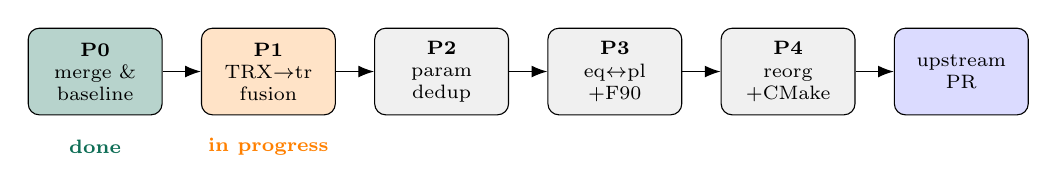
\begin{tikzpicture}[>={Latex[length=2mm]},
  ph/.style={draw, rounded corners, align=center, font=\scriptsize,
             minimum width=17mm, minimum height=11mm}]
  \node[ph, fill=ok!30]     (p0) at (0,0)    {\textbf{P0}\\ merge \&\\ baseline};
  \node[ph, fill=orange!22] (p1) at (2.2,0)  {\textbf{P1}\\ TRX$\to$tr\\ fusion};
  \node[ph, fill=gray!12]   (p2) at (4.4,0)  {\textbf{P2}\\ param\\ dedup};
  \node[ph, fill=gray!12]   (p3) at (6.6,0)  {\textbf{P3}\\ eq$\leftrightarrow$pl\\ +F90};
  \node[ph, fill=gray!12]   (p4) at (8.8,0)  {\textbf{P4}\\ reorg\\ +CMake};
  \node[ph, fill=blue!14]   (up) at (11.0,0) {upstream\\ PR};
  \draw[->] (p0)--(p1); \draw[->] (p1)--(p2); \draw[->] (p2)--(p3); \draw[->] (p3)--(p4); \draw[->] (p4)--(up);
  \node[font=\scriptsize\bfseries, text=ok]     at (0,-0.95)   {done};
  \node[font=\scriptsize\bfseries, text=orange] at (2.2,-0.95) {in progress};
\end{tikzpicture}
\end{center}
\footnotesize
\begin{itemize}
\item \textbf{P1} (now): Tasks 2--10 --- port \C{libnf}/\C{tr\_pnf}, validate \C{model\_pnf=1..4} vs bpsi \C{trx} @1e-10, archive \C{trx}/\C{trm}.
\item \textbf{P2}: de-duplicate shared params (\C{RR}/\C{RA}/\C{BB}\,\dots) into \C{plcomm}.
\item \textbf{P3}: \C{eq}$\leftrightarrow$\C{pl} interface + remaining F90-ification. \quad \textbf{P4}: directory reorg + CMake.
\item Then the \textbf{upstream} \C{myfork}$\to$\C{k-yoshimi/task} pull request.
\end{itemize}
\end{frame}

\begin{frame}{Repositories, links \& current result}
\footnotesize
\begin{tabular}{@{}p{45mm}p{26mm}p{37mm}@{}}
\toprule
Repo (click to open) & Role & State \\
\midrule
\href{https://github.com/ats-fukuyama/task}{\texttt{ats-fukuyama/task}} & GitHub backup (stale) & --- \\
\texttt{bpsi.nucleng.kyoto-u.ac.jp} & Kyoto main dev & base \texttt{fa9dd493} \\
\href{https://github.com/HengyuLi-Ozaki-lab/task/tree/kyoshimi-develop}{\texttt{HengyuLi-Ozaki-lab/task}} & \textbf{unified fork} & \texttt{kyoshimi-develop} @ \texttt{d1f7f9e7} \\
\href{https://github.com/HengyuLi-Ozaki-lab/task-merge/pull/1}{\texttt{HengyuLi-Ozaki-lab/task-merge}} & merge/test sandbox & PR \#1 (merged) \\
\bottomrule
\end{tabular}
\vspace{0.3em}
\begin{center}\scriptsize
$\hookrightarrow$ \href{https://github.com/HengyuLi-Ozaki-lab/task/blob/kyoshimi-develop/docs/2026-06-TASK-merge-and-TRX-report.md}{full engineering report}\quad
$\hookrightarrow$ \href{https://github.com/HengyuLi-Ozaki-lab/task/tree/kyoshimi-develop/docs/presentations}{these slides (.tex)}
\end{center}
\vspace{0.3em}
\begin{center}
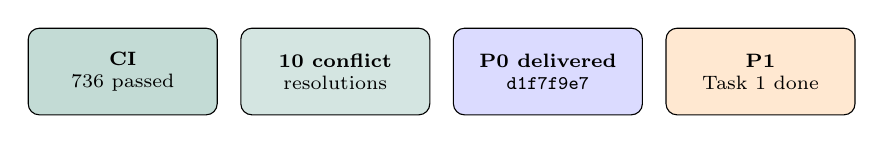
\begin{tikzpicture}[bg/.style={draw, rounded corners, align=center, font=\scriptsize,
                    minimum width=24mm, minimum height=11mm}]
  \node[bg, fill=ok!25]     at (0,0)   {\textbf{CI}\\ 736 passed};
  \node[bg, fill=ok!18]     at (2.7,0) {\textbf{10 conflict}\\ resolutions};
  \node[bg, fill=blue!14]   at (5.4,0) {\textbf{P0 delivered}\\ \texttt{d1f7f9e7}};
  \node[bg, fill=orange!18] at (8.1,0) {\textbf{P1}\\ Task 1 done};
\end{tikzpicture}
\end{center}
\vspace{0.3em}
\begin{center}\large\textbf{P0 delivered (CI \good{}); P1 underway.}\qquad\Large\textbf{Thank you.}\end{center}
\end{frame}

\end{document}
